
%(BEGIN_QUESTION)
% Copyright 2009, Tony R. Kuphaldt, released under the Creative Commons Attribution License (v 1.0)
% This means you may do almost anything with this work of mine, so long as you give me proper credit


Skummles "Continuous Fluid flow Measurment" kapittelet i afgv.pdf for spesifikt å besvare disse spørsmålene:
%Skim the ``Continuous Fluid Flow Measurement'' chapter in your {\it Lessons In Industrial Instrumentation} textbook to specifically answer these questions:

\vskip 10pt

Trykkbaserte strømningsmålere virker med å tvinge et fluid til å \textit{akselerere} eller \textit{deakselerere} mens det strømmer igjennom et rør. Dette gjør at det oppstår en trykkforsjell. Plukk ut noen av de forskjellige måleelementene (metoder) som brukes til å skape denne akselerasjonen eller deakselerasjonen. (hint. Venturirør er et eksempel)
%Pressure-based flowmeters work by forcing the fluid to {\it accelerate} or {\it decelerate} as it flows through a pipe, which causes a static pressure difference to develop.  Identify some of the different {\it flow elements} used to create the acceleration/deceleration inside a pipe (hint: a ``venturi tube'' is one example of a flow element creating a pressure differential).

\vskip 10pt
For hvert ev måleelementene finn ut om de virker med å akselerere eller deakselerere fluidet. Forklar hvorfor du tror det. 
%For each of the flow elements you identify, determine whether it works by fluid acceleration or by fluid deceleration, and explain your reasoning.

\vskip 10pt

I hvilken del av måleelementet er trykket størst, der hvor hastigheten er størst eller der hvor hastigheten er minst. (Hint. så på hvordan DP-cellen er tilkoblet. )
%In which region of a flow element is the pressure greatest, the region of {\it greatest velocity} or the region of {\it least velocity}?  Hint: the orientation of the DP transmitter's ``H'' and ``L'' ports is a clue!


\vskip 20pt \vbox{\hrule \hbox{\strut \vrule{} {\bf Suggestions for Socratic discussion} \vrule} \hrule}

\begin{itemize}
\item{} Identify different strategies for ``skimming'' a text, as opposed to reading that text closely.  Why do you suppose the ability to quickly scan a text is important in this career?
\end{itemize}

\underbar{file i04020}
%(END_QUESTION)





%(BEGIN_ANSWER)


%(END_ANSWER)





%(BEGIN_NOTES)

Flow elements creating an acceleration of the fluid:

\begin{itemize}
\item{} Venturi tube
\item{} Orifice plate
\item{} Flow nozzle
\item{} Segmental wedge
\item{} V-cone
\item{} Pipe elbow ({\it radial} acceleration)
\end{itemize}

\vskip 10pt

Flow elements creating a deceleration of the fluid:

\begin{itemize}
\item{} Pitot tube
\item{} Averaging pitot tube
\item{} Annubar
\item{} Target
\end{itemize}

\vskip 10pt

In accelerating element types, the ``H'' port of the DP transmitter connects to the region of widest flow profile (slowest velocity), while the ``L'' port connects to the region of narrowest flow profile (fastest velocity).

\vskip 10pt

In decelerating element types, the ``H'' port of the DP transmitter connects to the region of flow stagnation (slowest velocity), while the ``L'' port connects to the region of full flow profile (normal velocity).





\vfil \eject

\noindent
{\bf Summary Quiz:}

$$\includegraphics[width=15.5cm]{i04020x01.eps}$$

\noindent
This flowmeter measures fluid flow rate by:

\begin{itemize}
\item{} Creating vortices in the fluid
\vskip 5pt 
\item{} Accelerating the fluid
\vskip 5pt 
\item{} Ultrasonic sound wave propagation
\vskip 5pt 
\item{} Decelerating the fluid
\vskip 5pt 
\item{} Sensing turbine rotation
\vskip 5pt 
\item{} Electromagnetic induction
\end{itemize}

\vfil \eject

\noindent
{\bf Summary Quiz:}

$$\includegraphics[width=15.5cm]{i04020x02.eps}$$

\noindent
This flowmeter measures fluid flow rate by:

\begin{itemize}
\item{} Creating vortices in the fluid
\vskip 5pt 
\item{} Accelerating the fluid
\vskip 5pt 
\item{} Ultrasonic sound wave propagation
\vskip 5pt 
\item{} Decelerating the fluid
\vskip 5pt 
\item{} Sensing turbine rotation
\vskip 5pt 
\item{} Electromagnetic induction
\end{itemize}


%INDEX% Reading assignment: Lessons In Industrial Instrumentation, Continuous Fluid Flow Measurement (pressure-based)

%(END_NOTES)


